
\chapter{OBSERVER-BASED CONTROLS}
\label{chap:ObserverBasedControls}

This chapter assesses the viability of incorporating this research's state error, estimation, and control methods then applying the combined system to control the nutation and boom dynamics of TableSat.  All satellite modeling, state error calculations, estimation and control methods in this test is performed with the TSatPy software developed for this research.

\section{Sliding Mode Observer with Sliding Mode Controller}

In this simulation, a plant governed by the rigid body dynamics of Euler's Moment equations (Equation (\ref{eqn:DiscreteEulerMomentEquations})) is initialized to a 2 radian rotation about $0 \bs{i} +0.1 \bs{j} +1 \bs{k}$ with body-fixed angular velocities of $\omega = [0.01 \ -0.005 \ 0.2]^T$.

The Sliding Mode Observer is chosen as the observer and is configured estimator gains such that
\begin{equation}
  \begin{aligned}
    L_q &= 0.02, \bs{L}_{\omega} = \bs{I} \begin{bmatrix} 0.02 & 0.02 & 0.02 \end{bmatrix}^T \\
    K_q &= 0.001, \bs{K}_{\omega} = \bs{I} \begin{bmatrix} 0.001 & 0.001 & 0.001, \end{bmatrix}^T \\
    S_q &= 0.001, S_{\omega} = 0.001
  \end{aligned}
\end{equation}
The Sliding Mode Controller (Equation (\ref{eqn:sliding_mode_control})) is modified to act on the 5-DOF state error measurement such that
\begin{equation}
  \begin{aligned}
    \bs{M} &= \bs{M}_{q} + \bs{M}_{\omega} \\
    \bs{M}_{q} &= \left[- L_{q} \cos^{-1} (q_{0en}) \right] \bs{\hat{e}}_{en} + \left[ K_{q} sat \left( \frac{-2\cos^{-1} (q_{0en})}{S_q} \right) \right] \bs{\hat{e}}_{en} \\
    \bs{M}_{\omega} &= \bs{L}_{\omega} \bs{\omega}_e + \bs{K}_{\omega}\bs{1}_s \big(\bs{\omega}_e / S_{\omega} \big) \\
  \end{aligned}
\end{equation}
where the controller's state error quaternion $\bs{q}_e$ is decomposed into a rotation quaternion $\bs{q}_{er}$ and nutation quaternion  $\bs{q}_{en}$ such that
\begin{equation}
  \bs{q}_e = \bs{q}_{en} \otimes \bs{q}_{er}
\end{equation}
and $q_{0en}$ is the scalar component of $q_{en}$ and the $\bs{\hat{e}}_{en}$ is its Euler rotation axis.

The SMC's gains are chosen such that
\begin{equation}
  \begin{aligned}
    L_q &= 0.04, \bs{L}_{\omega} = \bs{I} \begin{bmatrix} 0.398 & 0.383 & 0.416 \end{bmatrix}^T \\
    K_q &= 0.04, \bs{K}_{\omega} = \bs{I} \begin{bmatrix} 0.440 & 0.510 & 0.316 \end{bmatrix}^T \\
    S_q &= 0.3, S_{\omega} = 0.140
  \end{aligned}
\end{equation}


The results from the simulated TableSat motion are shown in Figure \ref{fig:ObserverBasedControllerTruth}
\begin{figure}[H]
  \centerline{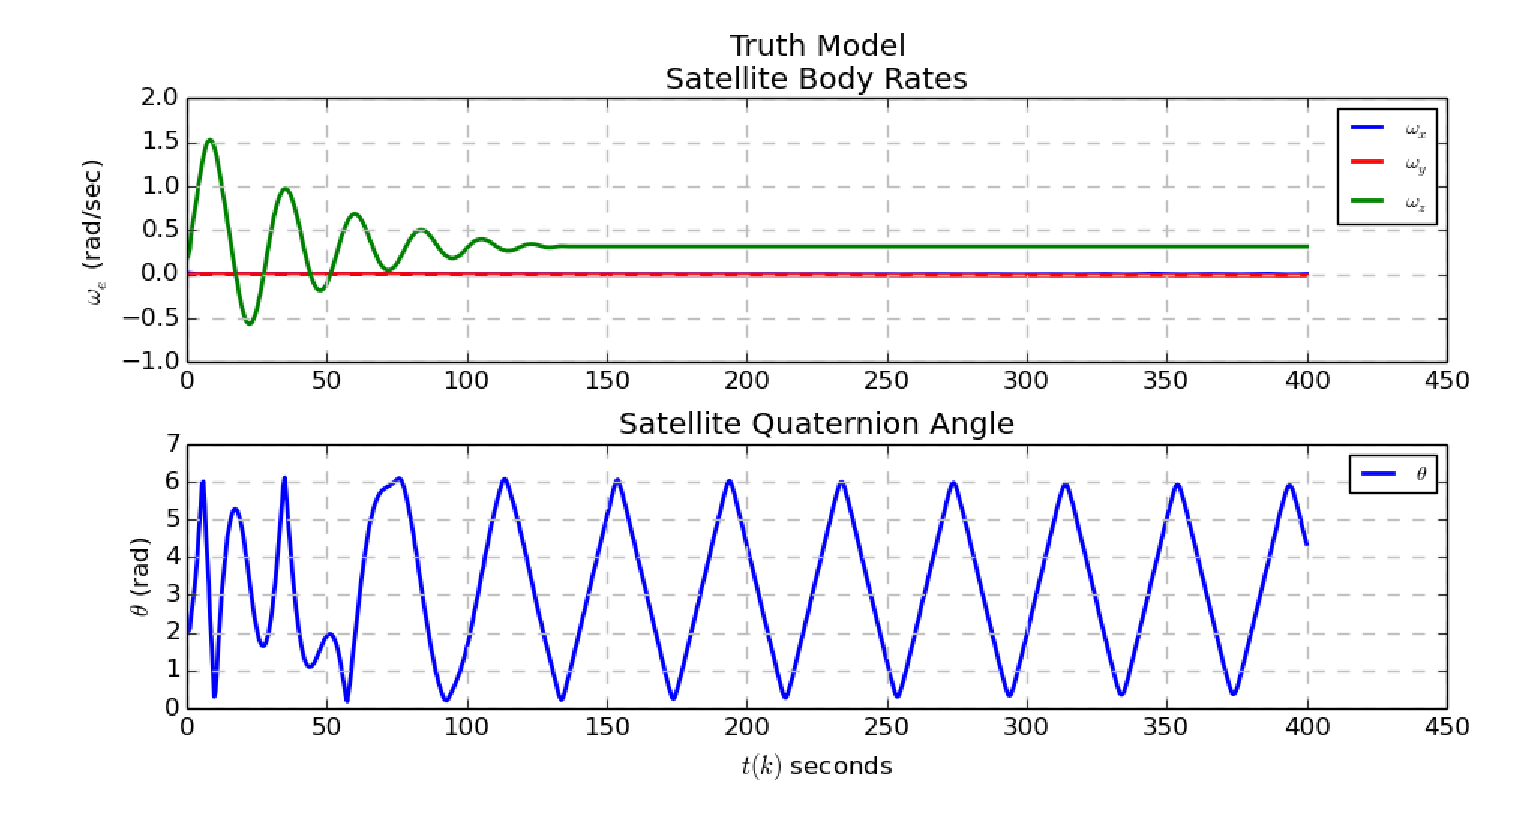
\psfig{file=figures/obc_01_truth.eps,width=6in}}
  \caption{Observer-Based Controller (Truth Model)}
  \label{fig:ObserverBasedControllerTruth}
\end{figure}

The body rates stabilize to the desired levels after approximately 125 seconds.  The ``Satellited Quaternion Angle'' quantifies the angular displacement between TableSat's current orientation and if its body-fixed axes were aligned with the inertial reference frame.

For a nutation and boom oscillation free spin-stabilized system, this method of measurement will provide a saw tooth pattern starting at 0 and climbing to $2\pi$ in the first rotation.  Although the satellite continues to rotate in the same direction through the second rotation, quaternion multiplication represents the angles as a decrease angle from $2\pi$ to 0 with the vector component inverted (not shown).

The attitude control for this simulation as seen in Figure \ref{fig:ObserverBasedControllerTruth} follows the expected pattern after the initial transient response although further inspection of the nutation angle as represented in the ``Attitude Error'' plot in Figure \ref{fig:ObserverBasedControllerSMC} shows a small but unstable growth which is not present in the attitude error of the estimator in Figure \ref{fig:ObserverBasedControllerSMO}.
\begin{figure}[H]
  \centerline{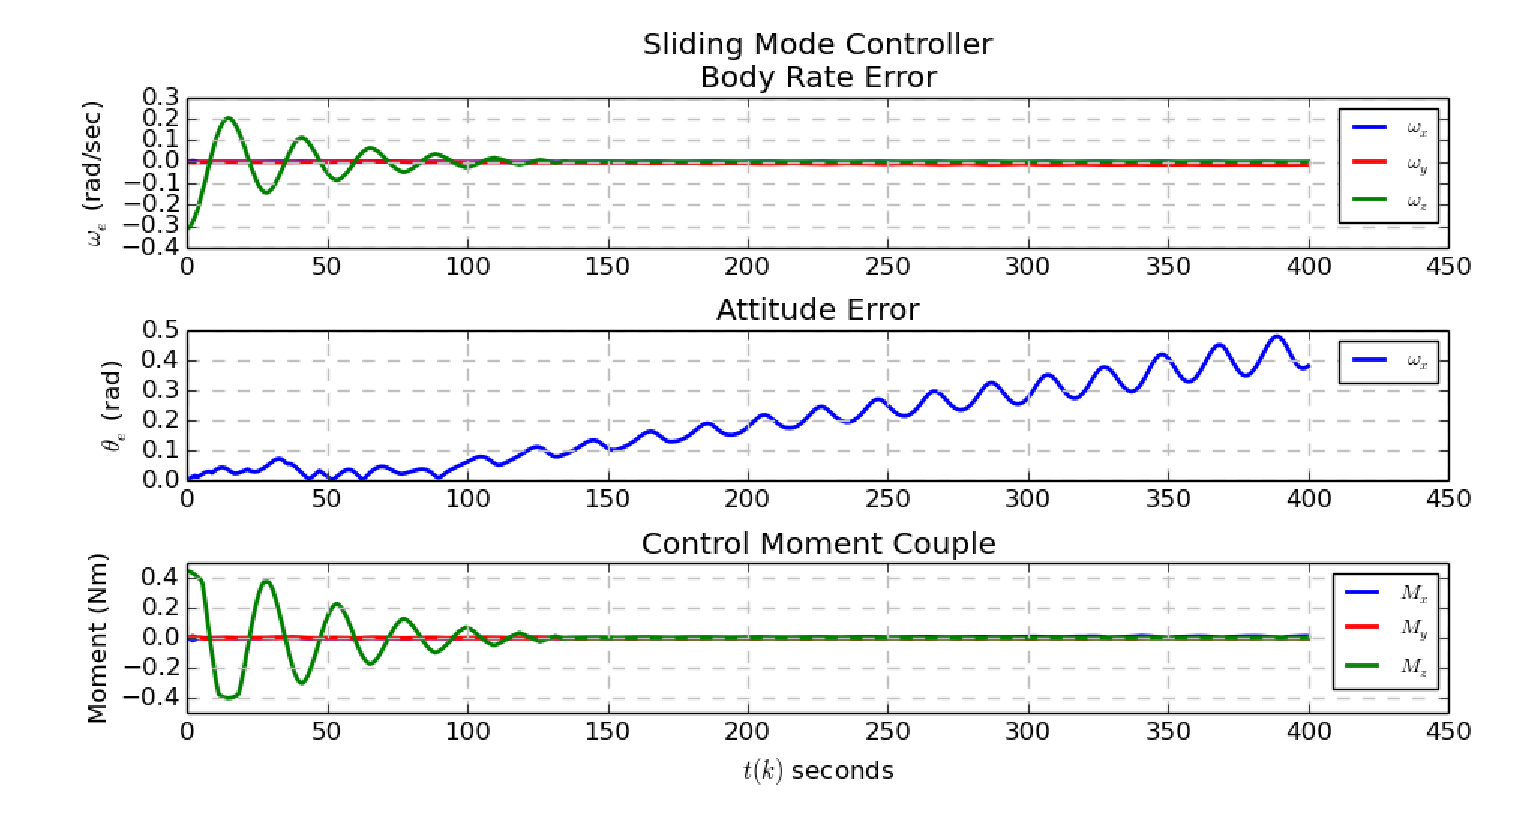
\psfig{file=figures/obc_01_smc.eps,width=6in}}
  \caption{Observer-Based Controller (SMC)}
  \label{fig:ObserverBasedControllerSMC}
\end{figure}

\begin{figure}[H]
  \centerline{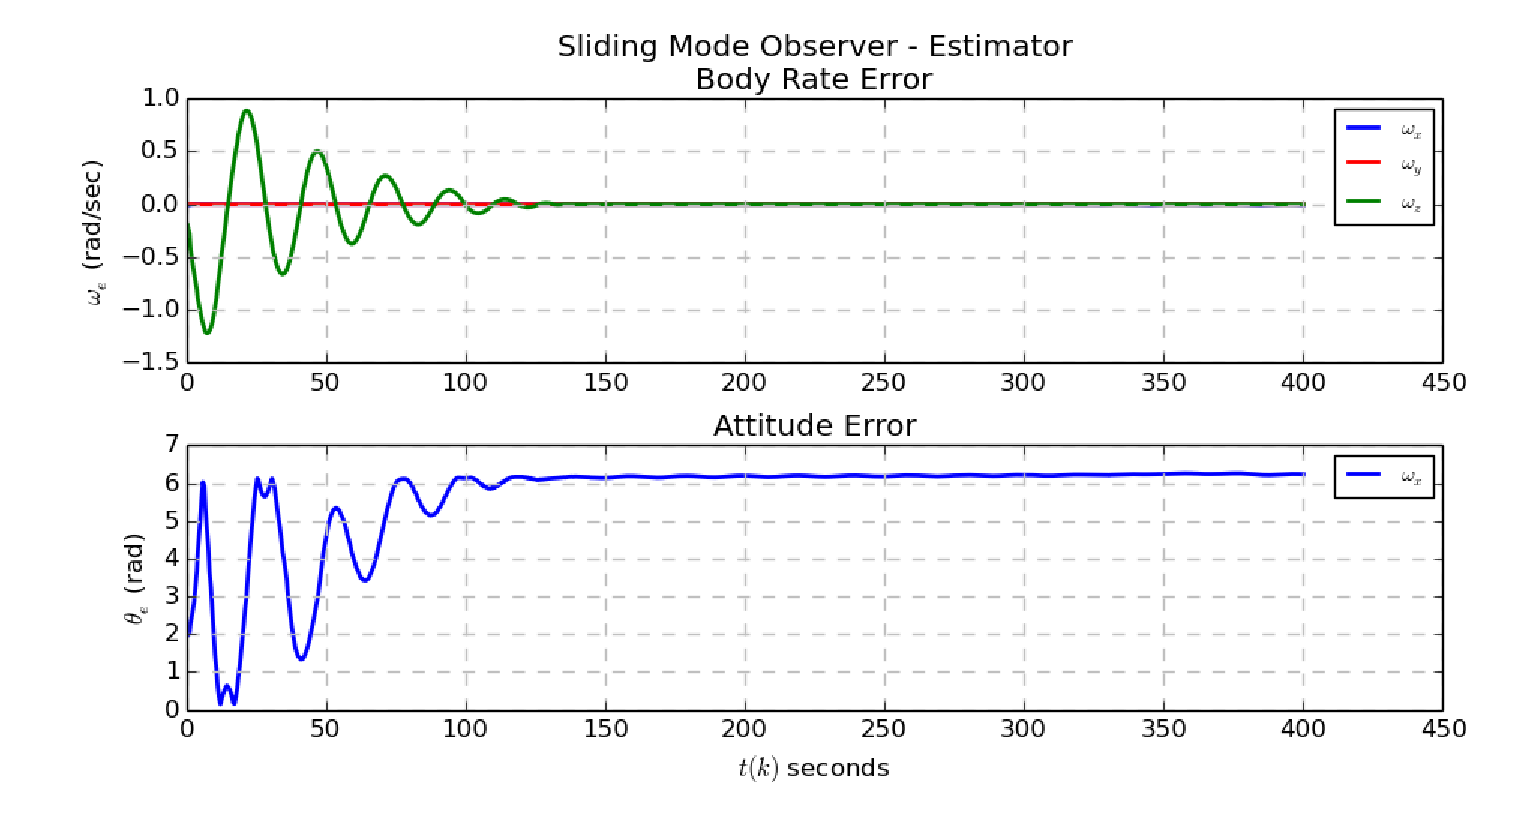
\psfig{file=figures/obc_01_smo.eps,width=6in}}
  \caption{Observer-Based Controller (SMO)}
  \label{fig:ObserverBasedControllerSMO}
\end{figure}

Sufficient control of the nutation is not found through manual gain selection in this observer-based controller configuration which restricts its ability to adequately control for nutation with the experimental TableSat IA.  This issue in conjunction with the insufficient nutation measurement resolution in the thee-axis magnetometer and limited nutation control with the two under powered fans currently prevents the successful testing of nutation control and boom dynamics.  Further study is recommended to address the gain selection and experimental model.

